\documentclass[a4paper,10pt,fleqn]{article}

\usepackage{a4wide,amsmath,amsthm,amssymb,bbm,fancyhdr}
\usepackage{ifthen,color,enumerate,comment,dsfont,pdfsync,framed,todonotes,enumitem}

\newcommand{\titre}[1]{\textbf{\textsc{#1}}}

\RequirePackage[T1]{fontenc}

\usepackage[latin1]{inputenc}
\usepackage{graphicx}
\usepackage{dsfont}
\usepackage{enumitem}
\newcommand{\eqsp}{\,}
\newcommand{\R}{\ensuremath{\mathbb{R}}}
\newcommand{\calF}{\mathcal{F}}
\newcommand{\rmd}{\mathrm{d}}
\newcommand{\N}{\mathbb{N}}
\newcommand{\rset}{\ensuremath{\mathbb{R}}}
\renewcommand{\P}{\ensuremath{\operatorname{P}}}
\newcommand{\bP}{\mathbb{P}}
\newcommand{\E}{\ensuremath{\mathbb{E}}}
\newcommand{\rme}{\ensuremath{\mathrm{e}}}
\newcommand{\calH}{\ensuremath{\mathcal{H}}}
\newcommand{\xset}{\ensuremath{\mathsf{X}}}
\newcommand{\V}{\ensuremath{\mathbb{V}}}
\newcommand{\Sb}{\ensuremath{\mathbb{S}}}
\newcommand{\gaus}{\ensuremath{\mathcal{N}}}
\newcommand{\HH}{\ensuremath{\mathcal{H}}}
\newcommand{\F}{\ensuremath{\mathcal{F}}}
\newcommand{\W}{\ensuremath{\mathcal{W}}}
\newcommand{\X}{\ensuremath{\mathcal{X}}}
\newcommand{\1}{\ensuremath{\mathbbm{1}}}
\newcommand{\dlim}{\ensuremath{\stackrel{\mathcal{L}}{\longrightarrow}}}
\newcommand{\plim}{\ensuremath{\stackrel{\mathrm{P}}{\longrightarrow}}}
\newcommand{\PP}{\ensuremath{\mathbb{P}}}
\newcommand{\p}{\ensuremath{\mathbb{P}}}
\newcommand{\eps}{\varepsilon}
\newcommand{\bE}{\mathbb{E}}
\newcommand{\pa}[1]{\left(#1\right)}
\newcommand{\hatk}{\widehat K}
\newcommand{\f}{\varphi}
\newcommand{\Id}{\textsf{Id}}
\newcommand{\bfU}{\mathbf{U}}
\newcommand{\bfX}{\mathbf{X}}
\newcommand{\bfs}{\mathbf{\Sigma}}
\newcommand{\bfA}{\mathbf{A}}
\newcommand{\bfV}{\mathbf{V}}
\newcommand{\bfB}{\mathbf{B}}
\newcommand{\bfI}{\mathbf{I}}
\newcommand{\bfD}{\mathbf{D}}
\newcommand{\bfK}{\mathbf{K}}
\newcommand{\argmin}{\mathop{\textrm{argmin}}}
\newcommand{\argmax}{\mathop{\textrm{argmax}}}
\newcommand{\crit}{\mathop{\textrm{crit}}}
\newcommand{\C}{\mathcal{C}}
\newcommand{\pc}{\pi_{\mathcal{C}}}


% Style


\newtheorem{theorem}{Theorem}


\begin{document}

\noindent Machine learning \hfill ISUP - Sorbonne Universit\'e \\
 2022-2023

\noindent\hrulefill

\begin{center}
\textsc{Introduction to supervised learning}
\end{center}
\hrulefill

\medskip


\section{Warm-up: Bayes classifier for scalar Gaussian mixtures}
Let $(X_i,Y_i)_{1\leqslant i\leqslant n}$ be independent variables in $\mathbb{R}\times \{0,1\}$. Assume that  $\mathbb{P}(Y_1 = 0) = 1/2$. Assume also that the distribution of $X_1$ given $\{Y_1= 0\}$ (resp. $\{Y_1= 1\}$) is Gaussian with mean $\mu_0$ (resp. $\mu_1$) and variance $1$. The probability density function of $X_1$ is written $g$. Write
$$
g_0: x \mapsto (2\pi)^{-1/2}\exp(-(x-\mu_0)^2/2)\quad\mathrm{and} \quad g_1: x \mapsto (2\pi)^{-1/2}\exp(-(x-\mu_1)^2/2)\eqsp.
$$
\begin{figure}[h!]
\begin{center}
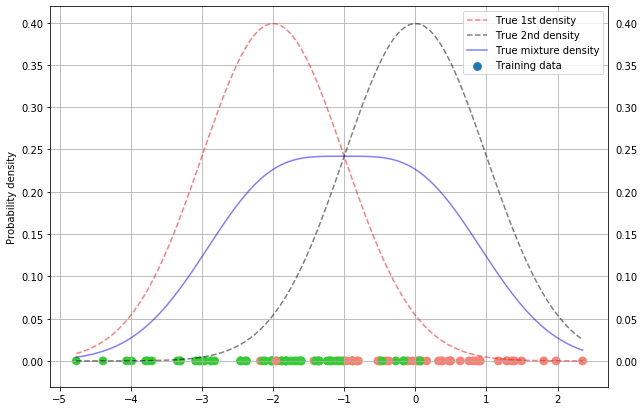
\includegraphics[scale=0.3]{mu0_mum2.png}
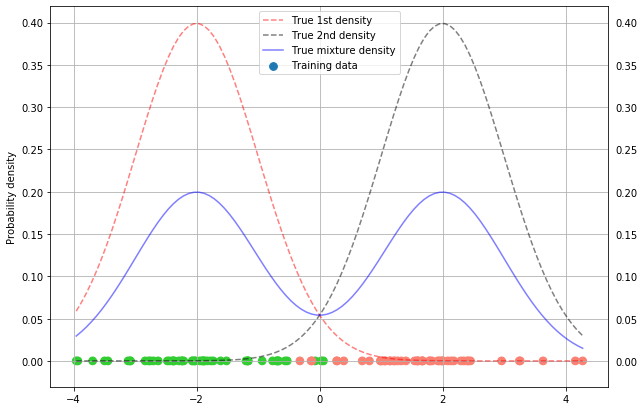
\includegraphics[scale=0.3]{mu2_mum2.png}
\caption{Samples and density when   $\mu_0 = -2$ et $\mu_1 = 0$ (left) and $\mu_0 = -2$ and $\mu_1 = 2$ (right).}
\end{center}
\end{figure}

\begin{enumerate}
\item Recall the definition of the Bayes classifier.

\vspace{.2cm}

{\em The Bayes classifier $h_*: \mathbb{R}\to \{0,1\}$ minimizes the missclassification error:
$$
h_{*} \in \mathrm{Argmin}_{h:\rset\to \{0,1\}}\left\{\bP(h(X)\neq Y)\right\}\eqsp.
$$
It satisfies $h_{*}(X) = 1$ if and only if $\bP(Y=1|X)> \bP(Y=0|X)$.}

\item Using Bayes rule, show that  $h_*$ depends only on $g_1/g_0$.

\vspace{.2cm}

{\em  By Bayes formula, $\bP(Y=1|X) = \bP(Y=1)g_1(X)/g(X)$, which yields
$$
\frac{\bP(Y=1|X)}{\bP(Y=0|X)} = \frac{g_1(X)}{g_0(X)}\eqsp.
$$
Then, $h_*(X) = 1$ if and only if $g_1(X)/g_0(X)>1$.
}

\item Show that the Bayes classifier uses the mean between  $\mu_0$ and  $\mu_1$ to classify samples.

\vspace{.2cm}

{\em $h_*(X) = 1$ if and only if  $\log g_1(X) - \log g_0(X)>0$, so that, assuming without loss of generality that $\mu_1>\mu_0$:
\begin{align*}
h_*(X) = 1 & \Leftrightarrow (X-\mu_0)^2 - (X-\mu_1)^2>0\,,\\
& \Leftrightarrow 2 (\mu_1-\mu_0)X + \mu_0^2 - \mu_1^2>0\,,\\
&\Leftrightarrow X> \frac{\mu_1^2 - \mu_0^2}{2(\mu_1-\mu_0)}\,,\\
& \Leftrightarrow X> \frac{\mu_1 + \mu_0}{2}\eqsp.
\end{align*}
This criterion can lead to very poor performance if means are close (see Figure~1).}
\end{enumerate}



\section{Bayes classifier}
\subsection{Exercice 1}
Assume that $(X,Y)\in\mathbb{R}\times\{0,1\}$ is defined on $(\Omega,\mathcal{F},\mathbb{P})$ with $\mathbb{P}(Y=1) = \pi \in(0,1)$.  Assume that conditionally on $\{Y=0\}$ (resp. $\{Y=1\}$) $X$ has a uniform distribution on $[0,\theta]$ with $\theta\in(0,1)$ (resp. on $[0,1]$). Compute $\eta(X) = \mathbb{P}(Y=1 |X)$.

\vspace{.2cm}

{\em
Let $g$ be the probability density function of $X$. For any measurable set $A$,
\begin{align*}
\mathbb{P}(X\in A) &= \mathbb{P}(Y=0)\mathbb{P}(X\in A|Y=0) + \mathbb{P}(Y=1)\mathbb{P}(X\in A|Y=1)\,,\\
&= (1-\pi) \theta^{-1}\int \1_A(x)\1_{[0,\theta]}(x) \rmd x + \pi \int \1_A(x)\1_{[0,1]}(x) \rmd x\,,\\
&= \int \1_A(x)\left\{ (1-\pi) \theta^{-1}\1_{[0,\theta]}(x) + \pi\1_{[0,1]}(x)\right\} \rmd x\,.
\end{align*}
Therefore, $g:x\mapsto  (1-\pi) \theta^{-1}\1_{[0,\theta]}(x) + \pi\1_{[0,1]}(x)$. Then, using Bayes rules and writing $g_1$ the probability density of the distribution of $X$ given $\{Y=1\}$,
$$
\eta(X) = \mathbb{P}(Y=1 |X) = \frac{ \mathbb{P}(Y=1)g_1(X)}{g(X)} = \frac{\pi \1_{[0,1]}(X)}{(1-\pi) \theta^{-1}\1_{[0,\theta]}(X) + \pi\1_{[0,1]}(X)}
$$

}

\subsection{Exercice 2}
Assume that $(X,Y)\in\mathbb{R}\times\{0,1\}$ is defined on $(\Omega,\mathcal{F},\mathbb{P})$. The distribution of $X$ is written $\mu$ and $\eta(X) = \mathbb{P}(Y=1|X) = X(X+\theta)^{-1}$ where $\theta>0$. Compute the Bayes classifier $h^*$ in this setting and prove that
$$
R(h^*) = \bP(h^*(X)\neq Y) = \int \{\eta(x) \wedge (1-\eta(x))\}\mu(\rmd x)\,.
$$
Compute $R(h^*)$ when $\mu$ is the uniform distribution on $[0,\alpha \theta]$, $\alpha>1$. 

\subsection{Exercice 3}
Assume that $(X,Y)\in\mathbb{R}\times\{0,1\}$ is defined on $(\Omega,\mathcal{F},\mathbb{P})$. Using $\omega_0, \omega_1 >0$, with $\omega_0+\omega_1 = 1$, we  consider the weighted risk:
$$
\mathsf{R}(h) = \bE[2\omega_Y \mathds{1}_{Y\neq h(X)}]\,.
$$
 Compute the Bayes classifier and its associated risk.

\section{Additional exercises}
\subsection{Plug-in classifier}
Let $(X,Y)\in\rset^d\times\{-1;1\}$ be random variables defined on the same probability space $(\Omega,\calF,\bP)$.
For any classifier $h:\mathcal{X}\to \{-1,1\}$, define its classification error by
$$
R(h)=\bP(Y\neq h(X))\eqsp.
$$
The best classifier in terms of the classification error $R$ is the Bayes classifier
$$
h_{*}(x)={\rm sign}(\eta(x)-1/2)\eqsp,
$$
where
$$
\eta(X) = \mapsto\bP(Y=1|X)\eqsp.
$$
Given $n$ independent couples $\{(X_i,Y_i)\}_{1\leqslant i \leqslant n}$ with the same distribution as $(X,Y)$, an empirical surrogate for $h_{*}$ is obtained from a possibly nonparametric estimator $\widehat \eta_n$ of $\eta$:
$$
\widehat h_n: x\mapsto {\rm sign}(\widehat \eta_n(x)-1/2)\eqsp.
$$
\begin{enumerate}
\item Prove that for any classifier $h:\mathcal{X}\to \{-1,1\}$,
$$
\bP(Y\neq h(X)|X) = (2\eta(X)-1)\1_{h(X)=-1}+1-\eta(X)
$$
and
$$
R(h)-R(h_{*})=2\bE \left[\left|\eta(X)-\frac{1}{2}\right|\eqsp\1_{h(X)\neq h_*(X)}\right]\eqsp.
$$
%
%\vspace{.2cm}
%
%{\em
%For all $x\in\xset$,
%\begin{align*}
%\bP\left(Y \neq h(X) | X\right)_{|X=x} & = \bP\left(Y=-1, h(X) = 1 |X\right)_{|X=x} + \bP\left(Y=1, h(X) = -1 |X\right)_{|X=x}\eqsp,\\
%& = \1_{h(x) = 1} \bP\left(Y=-1 |X\right)_{|X=x} + \1_{h(x) = -1} \bP\left(Y=1 |X\right)_{|X=x}\eqsp,\\
%& = \1_{h(x) = -1} (2\eta(x) - 1) + 1 - \eta(x)\eqsp.
%\end{align*}
%Let $\widetilde X$ be a random variable  independent of $X$ and with the same distribution as $X$. Then, 
%\begin{align*}
%R(h) - R(h_*) & = \bE\left[\bP\left(Y \neq h(X) | X=\widetilde X\right) - \bP\left(Y \neq h_*(X) | X=\widetilde X\right)\middle|X\right]\eqsp,\\
%& =  \bE\left[(2\eta(\widetilde X)-1) \left(\1_{h(\widetilde X) = -1} - \1_{h_*(\widetilde X) = -1} \right)\middle|X\right]\eqsp,\\
%& =  \bE\left[\1_{h_*(\widetilde X) \neq h(\widetilde X)} \left( (2\eta(\widetilde X)-1) \1_{h_*(\widetilde X)=1} - (2\eta(\widetilde X)-1) \1_{h_*(\widetilde X)=-1} \right)\middle|X\right]\eqsp,\\
%& = 2\bE\left[\left| \eta(X) - 1/2 \right| \1_{h_*(X) \neq h(X)}\right]\eqsp.
%\end{align*}
%}
\item Prove that 
$$
|\eta(x)-1/2|\1_{\widehat h_n(x)\neq h_{*}(x)}\leqslant |\eta(x)-\widehat \eta_n(x)|\1_{\widehat h_n(x)\neq h_{*}(x)}\eqsp,
$$
where
$$
\widehat h_n:x \mapsto{\rm sign}(\widehat \eta_n(x)-1/2)\eqsp.
$$
Deduce that 
$$
R(\widehat h_n)-R(h_*)\leqslant 2\|\widehat \eta_n-\eta\|_{\mathrm{L}^2(\bP_X)}\eqsp,
$$
where $\bP_X$ is the distribution of $X$.
%\vspace{.2cm}
%
%{\em
%Note that 
%\[
%\{x\in\xset\eqsp;\eqsp \widehat h_n(x) \neq h_*(x)\} =  \{x\in\xset\eqsp;\eqsp \eta(x) \geqslant 1/2\eqsp,\eqsp\widehat\eta_n(x) \leqslant 1/2\}\cup\{x\in\xset\eqsp;\eqsp \eta(x) \leqslant 1/2\eqsp,\eqsp\widehat \eta_n(x) \geqslant 1/2\}\eqsp.
%\]
%For all $x\in \{x\in\xset\eqsp;\eqsp \eta(x) \geqslant 1/2\eqsp,\eqsp\widehat\eta_n(x) \leqslant 1/2\}$,
%\begin{align*}
%|\eta(x) - \widehat\eta_n(x)| = \eta(x) - \widehat\eta_n(x) \geqslant \eta(x) -1/2\eqsp
%\end{align*}
%On the other hand, for all $x\in\{x\in\xset\eqsp;\eqsp \eta(x) \leqslant 1/2\eqsp,\eqsp\widehat \eta_n(x) \geqslant 1/2\}$,
%\begin{align*}
%|\eta(x) - \widehat\eta_n(x)| = \widehat\eta_n(x) - \eta(x) \geqslant 1/2 - \eta(x)\eqsp.
%\end{align*}
%Therefore, for all $x\in\xset$,
%\begin{align*}
%|\eta(x) - 1/2| \1_{\widehat h_n(x) \neq h_*(x)}\leq |\eta(x) - \widehat \eta_n(x)| \1_{\widehat h_n(x) \neq h_*(x)}.
%\end{align*}
%By the first question and Cauchy-Schwarz inequality, 
%\begin{align*}
%R(\widehat h_n) - R(h_*) & = 2  \bE \left[ \left| \eta(X) - 1/2 \right| \1_{h_*(X) = \widehat h_n(X)}  \right] \leqslant 2 \bE \left[ \left|\eta(X) - \widehat \eta_n(X) \right| \1_{\widehat h_n(X) \neq h_*(X)}  \right] \leqslant 2 \|\eta - \widehat \eta_n \|_{\mathrm{L}^2(\bP_X)}\eqsp.
%\end{align*}
%}
\end{enumerate}
%
%%\section*{Logistic Regression}
%%The \emph{logistic model} assumes that the random variables  $(X,Y)\in \rset^p\times\{0,1\}$ are such that
%%\begin{equation}\label{eq:logistic}
%%\bP(Y=1|X)={\exp\left(\langle \beta^*,X\rangle\right)\over 1+\exp\left(\langle \beta^*,X\rangle\right)}\eqsp,
%%\end{equation}
%%with $\beta^*\in\mathbb{R}^d$. In this case, for all $x\in\rset^d$, $\bP(Y=1|X)|_{X=x}>1/2$ if and only if $\langle \beta^*,x\rangle>0$, so
%%the frontier between $\left\{x\eqsp;\eqsp h_{*}(x)=1\right\}$ and $\left\{x\eqsp ;\eqsp h_{*}(x)=0\right\}$ is an hyperplane, with orthogonal
%%direction $\beta^*$. The unknown parameter $\beta^*$ may be estimated  by maximizing the conditional likelihood of $Y$ given $X$
%%\begin{align*}
%%\widehat \beta_n\in\mathrm{argmax}_{\beta\in\mathbb{R}^{d}}
%%\prod_{i=1}^n \left[ \left( \frac{\exp\left(\langle
%%	\beta,x_{i}\rangle\right)}{1+\exp\left(\langle
%%	\beta,x_{i}\rangle\right)}\right)^{Y_{i}}
%%\left(\frac{1}{1+\exp\left(\langle
%%	\beta,x_{i}\rangle\right)}\right)^{1- Y_{i}} \right] ,
%%\end{align*}
%%to define the empirical classifier
%%\[
%%\widehat h_{n}: x \mapsto \1_{\langle \widehat\beta_n,x\rangle>0}\eqsp.
%%\]
%%\begin{enumerate}
%%\item Compute the gradient and the Hessian $H_{n}$ of
%%\[
%%\ell_{n}:\beta \mapsto -\sum_{i=1}^n\left[Y_{i}\langle x_{i},\beta\rangle-\log(1+\exp(\langle x_{i},\beta\rangle))\right]\eqsp.
%%\]
%%%are given by
%%%\begin{align*}
%%%\nabla\ell_{n}(\beta)= -\sum_{i=1}^n\left(Y_{i}- \frac{
%%%	e^{\langle x_{i},\beta\rangle}}{1+e^{\langle
%%%		x_{i},\beta\rangle}}\right)x_{i} \quad\textrm{and} \quad
%%%H_{n}(\beta)=\sum_{i=1}^n\frac{e^{\langle
%%%		x_{i},\beta\rangle}}{\left(1+e^{\langle
%%%		x_{i},\beta\rangle}\right)^2}\,x_{i}x_{i}^T\eqsp.
%%%\end{align*}
%%What can be said about the function $\ell_{n}$ when for all $\beta\in\rset^d$, $H_{n}(\beta)$ is nonsingular? This assumption is supposed to hold in the following questions.
%%
%%\vspace{.2cm}
%%
%%{\em
%%Since for all $u\in\rset^d$, $\nabla_{\beta} \langle u, \beta \rangle = u$, 
%%\[
%%\nabla \ell_n(\beta) = - \sum_{i=1}^n Y_i x_i + \sum_{i=1}^n \frac{\exp(\langle x_{i},\beta\rangle)}{1  + \exp(\langle x_{i},\beta\rangle)} x_i\eqsp.
%%\]
%%On the other hand, for all $1\leqslant i \leqslant n$ and all $1 \leqslant j \leqslant d$,
%%\[
%%\partial_j \left( \frac{\exp(\langle x_{i},\beta\rangle)}{1  + \exp(\langle x_{i},\beta\rangle)} x_i \right) = \frac{\exp(\langle x_{i},\beta\rangle)}{(1  + \exp(\langle x_{i},\beta\rangle))^2} x_{ij}x_i\eqsp,
%%\]
%%where $x_{ij}$ is the $j$th component of $x_i$. Then
%%\[
%%\big(H_n(\beta)\big)_{\ell j} = \sum_{i=1}^n \frac{\exp(\langle x_{i},\beta\rangle)}{(1  + \exp(\langle x_{i},\beta\rangle))^2} x_{ij}x_{i \ell}\eqsp,
%%\]
%%that is,
%%\[
%%H_n(\beta) = \sum_{i=1}^n \frac{\exp(\langle x_{i},\beta\rangle)}{(1  + \exp(\langle x_{i},\beta\rangle))^2} x_{i} x_{i}'\eqsp.
%%\]
%%%Note that $H_n(\beta)$ is the Gram matrix 
%%%\[
%%%H_n(\beta)   = \langle \tilde{x}_i, \tilde{x}_j \rangle,
%%%\]
%%%where 
%%%\[
%%%\tilde{x}_i = x_i \frac{\exp(\langle x_{i},\beta\rangle/2)}{1  + \exp(\langle x_{i},\beta\rangle)}\eqsp.
%%%\]
%%$H_n(\beta)$ is a semi positive definite matrix, which implies that $\ell_n(\beta)$ is convex. If we assume that $H_n$ is nonsingular, $\ell_n$  is strictly convex.
%%}
%%\item Prove that there exists $\widetilde \beta_n\in\rset^d$ such that $\|\widetilde \beta_n-\beta^*\|\leq \|\widehat \beta_n-\beta^*\|$ and
%%\[
%%\widehat \beta_n-\beta^*=-H_{n}(\widetilde \beta_n)^{-1}\nabla \ell_{n}(\beta^*)\eqsp.
%%\]
%%
%%\vspace{.2cm}
%%
%%{\em
%%Using a Taylor expansion between $\beta^{\star}$ and $\widehat{\beta}_n$, there exists $\tilde{\beta}_n \in B(\beta^{\star}, \|\widehat{\beta}_n - \beta^{\star}\|)$ such that 
%%\[
%%\nabla \ell_n(\widehat{\beta}_n) = \nabla \ell_n(\beta^{\star}) + H_n(\tilde{\beta}_n) ( \hat{\beta}_n - \beta^{\star})\eqsp. 
%%\]
%%By definition, $\ell_n(\widehat{\beta}_n) = 0$. Therefore, 
%%\[
%%\widehat{\beta}_n - \beta^{\star} = - H_n(\tilde{\beta}_n)^{-1} \nabla \ell_n(\beta^{\star})\eqsp,
%%\]
%%where $H_n(\tilde{\beta}_n)^{-1}$ exists since $H_n(\tilde{\beta})$ is assumed to be non-singular for all $\beta$.
%%}
%%\end{enumerate}
%%In the following it is assumed that the $(x_{i})_{1\leqslant i\leqslant n}$ are uniformly bounded, $\widehat \beta_n\to \beta^*$ a.s. and that there exists a continuous and nonsingular function $H$ such that $n^{-1}H_{n}(\beta)$ converges to $H(\beta)$, uniformly in a ball around $\beta^*$.
%%\begin{enumerate}  \setcounter{enumi}{2}
%%\item Define for all $1\leqslant i \leqslant n$, $p_{i}(\beta)=e^{\langle x_{i},\beta\rangle}/ \left(1+e^{\langle x_{i},\beta\rangle}\right)$. Check that
%%\begin{align*}
%%\bE \left[e^{-n^{-1/2}\langle t,\nabla\ell_{n}(\beta^*)\rangle}\right]& =\prod_{i=1}^n \left({1-p_{i}(\beta^*)+p_{i}(\beta^*)e^{\langle t,x_{i}\rangle/\sqrt{n}}}\right) e^{-p_{i}(\beta^*)\langle t,x_{i}\rangle/\sqrt{n}}\eqsp, \\
%%&=\exp\left(\frac{1}{2}t^T\left(n^{-1}H_{n}(\beta^*)\right)t+O(n^{-1/2})\right)\eqsp.
%%\end{align*}
%%
%%\vspace{.2cm}
%%
%%{\em For all $t\in\rset^d$,
%%\begin{align*}
%% \bE \left[ \exp\left( - \frac{1}{\sqrt{n}} \langle t, \nabla \ell_n(\beta^{\star}) \rangle \right) \right] = & \prod_{i=1}^n \bE \left[ \exp\left( \frac{1}{\sqrt{n}} (Y_i - p_i(\beta^{\star}) )\langle x_i, t \rangle \right) \right]\eqsp,\\
%%= & \prod_{i=1}^n \left[ \left( 1 - p_i(\beta^{\star}) +  p_i(\beta^{\star}) \exp\left( \frac{1}{\sqrt{n}} \langle x_i, t \rangle \right) \right) \exp \left( - \frac{ p_i(\beta^{\star})}{\sqrt{n}} \langle x_i, t \rangle \right) \right]\eqsp.
%%\end{align*}
%%Note that 
%%\[
%%\log \left( 1 - p_i + p_i \exp(u/\sqrt{n}) \right) =  \log\left( 1 + p_i \frac{u}{\sqrt{n}} + p_i \frac{u^2}{2n} + \textrm{O} \left( n^{-3/2} \right)\right)\\
%% = p_i \frac{u}{\sqrt{n}} + \frac{p_i u^2}{2n} - \frac{p_i^2 u^2}{2n} + \textrm{O} \left( n^{-3/2} \right)\eqsp.
%%\]
%%Finally, 
%%\[
%%\bE \left[ \exp\left( - \frac{1}{\sqrt{n}} \langle t, \nabla \ell_n(\beta^{\star}) \rangle \right) \right] = 
%%\exp\Bigg( \frac{1}{2n} \underbrace{\sum_{i=1}^n p_i(\beta^{\star}) (1 - p_i(\beta^{\star})) \langle t, x_i \rangle^2}_{t^T H_n(\beta^{\star}) t} + \textrm{O}(n^{-1/2})\Bigg)\eqsp.
%%\]
%%}
%%\item What is the asymptotic distribution of $-n^{-1/2}\nabla\ell_{n}(\beta^*)$ and of $\sqrt{n}(\widehat \beta_n-\beta^*)$?
%%
%%\vspace{.2cm}
%%
%%{\em
%%% Recall that for a vector-valued random variable X, the moment-generating function is defined as 
%%%\begin{align*}%
%%%M_X(t) = \bE \left[ \exp\left( \langle t, X \rangle \right) \right].
%%%\end{align*}
%%%In particular, we know that if $X \sim \mathcal{N}(\mu, \Sigma)$ then 
%%%\begin{align*}
%%%M_X(t) = \bE \left[ \exp \left( \langle t, \mu + \frac{1}{2} \Sigma t \rangle \right) \right].
%%%\end{align*}
%%%A convergence theorem states that if, for all $t$, $M_{X_n}(t) \to M_X(t)$ then $X_n \to X$ in distribution. 
%%For all $t\in\rset^d$, since $n^{-1} H_n(\beta^{\star}) \to_{n\to \infty} H(\beta^{\star})$,
%%\[
%%\bE \left[ \exp\left( - \frac{1}{\sqrt{n}} \langle t, \nabla \ell_n(\beta^{\star}) \rangle \right) \right] \to_{n\to \infty}  \exp\Bigg( \frac{1}{2} t^T H(\beta^{\star}) t \Bigg)\eqsp.
%%\]
%%Therefore, $-\nabla \ell_n(\beta^{\star}) / \sqrt{n}$ converges in distribution to  $Z \sim \mathcal{N}(0, H(\beta^{\star}))$. On the other hand, 
%%\begin{align*}
%%\sqrt{n} (\widehat{\beta}_n - \beta^{\star}) = - \left( \frac{1}{n} H_n(\tilde{\beta}_n) \right)^{-1} \frac{1}{\sqrt{n}} \nabla \ell_n(\beta^{\star})\eqsp.
%%\end{align*}
%%As for all $n\geqslant 1$, $\tilde{\beta}_n \in B(\beta^{\star}, \|\widehat{\beta}_n - \beta^{\star}\|)$, $\tilde{\beta}_n$ converges to  $\beta^{\star}$ almost surely as $n$ grows to infinity. Hence, almost surely
%%\[
%%\left( \frac{1}{n} H_n(\tilde{\beta}_n) \right)^{-1} \to H(\beta^{\star})^{-1}
%%\]
%%and, by Slutsky lemma, $\sqrt{n} (\widehat{\beta}_n - \beta^{\star})$  converges in distribution to  $Z \sim \mathcal{N}(0,  H(\beta^{\star})^{-1})$.
%%}
%%\item For all $1\leqslant j \leqslant d$ and all $\alpha\in(0,1)$, propose a confidence interval $\mathcal{I}_{n,\alpha}$ such that $\beta^*_{j}\in \mathcal{I}_{n,\alpha}$ with asymptotic probability $1-\alpha$.
%%
%%\vspace{.2cm}
%%
%%{\em
%%According to the last question, $\sqrt{n} ( \widehat{\beta}_j - \beta^{\star}_j) $ converges in distribution to a centered Gaussian random variable with variance $(H(\beta^{\star})^{-1})_{jj}$. On the other hand, almost surely,
%%\begin{align*}
%%\widehat{\sigma}_{n,j}^2 = (n H_n(\widehat{\beta}_n)^{-1})_{jj} \to_{n\to \infty} (H(\beta^{\star})^{-1})_{jj}\eqsp.
%%\end{align*}
%%Then, 
%%\begin{align*}
%%\sqrt{\frac{n}{\widehat{\sigma}_{n,j}^2}} (\widehat{\beta}_{n,j} - \beta^{\star}_j ) \to_{n\to \infty} \mathcal{N}(0,1).
%%\end{align*}
%%An asymptotic confidence interval $\mathcal{I}_{n,\alpha}$ of level $1-\alpha$ is then given by
%%\begin{align*}
%%\mathcal{I}_{n,\alpha} = \left[ \widehat{\beta}_{n,j} - z_{1-\alpha/2} \sqrt{\frac{\widehat{\sigma}^2_{n,j}}{n}}\eqsp,\eqsp \widehat{\beta}_{n,j} + z_{1-\alpha/2} \sqrt{\frac{\widehat{\sigma}^2_{n,j}}{n}}  \right],
%%\end{align*}
%%where $z_{1- \alpha/2}$ is the quantile of order $1- \alpha/2$ of $\mathcal{N}(0, 1)$.
%%}
%%\item  Propose a confidence ellipsoid $\mathcal{E}_{n,\alpha}$ such that the probability that $\beta^*\in \mathcal{E}_{n,\alpha}$ is asymptotically $1-\alpha$.
%%%
%%%\vspace{.2cm}
%%%
%%%{\em 
%%%Similarly to the previous question, we have
%%%\begin{align*}
%%%\sqrt{n} \left( \frac{1}{n} H_n(\widehat{\beta})\right)^{1/2} (\widehat{\beta} - \beta^{\star}) \to \mathcal{N}(0,I), 
%%%\end{align*}
%%%which leads to the following confidence ellipsoid of level $1-\alpha$
%%%\begin{align*}
%%%\mathcal{E}_{n,\alpha} = \widehat{\beta} + \frac{1}{\sqrt{n}} \left( \frac{1}{n} H_n(\widehat{\beta})\right)^{-1/2} B(0, r_{1 - \alpha}),
%%%\end{align*}
%%%where $B(0, r_{1 - \alpha})$ is the confidence ball of level $1-\alpha$ for the multivariate Gaussian $\mathcal{N}(0, I)$.
%%%}
%%\end{enumerate}
%%
%%\section*{K-means algorithm}
%%The K-means algorithm is a procedure which aims at partitioning a data set into $K$ distinct, non-overlapping clusters.
%%Consider $n\geqslant 1$ observations $(X_{1},\ldots,X_{n})$ taking values in $\mathbb{R}^p$.
%%The $K$-means algorithm seeks to minimize over all partitions $C = (C_{1},\ldots,C_{K})$ of $\{1,\ldots,n\}$ the following criterion
%%\[
%%\textrm{crit}(C)=\sum_{k=1}^K{1\over |C_{k}|}\sum_{a,b\in C_{k}} \|X_{a}-X_{b}\|^2\,,
%%\]
%%where for all $1\leqslant i\leqslant n$, $1\leqslant k\leqslant K$, $i\in C_k$ if and only if $X_i$ is in the $k$-th cluster.
%%\begin{enumerate}
%%\item Define the distance between two clusters $1\leqslant i,j\leqslant K$ as 
%%\[
%%d(C_i,C_j) = \sum_{a\in C_i\cup C_j}\|X_{a}-\bar{X}_{C_{i}\cup C_j}\|^2 - \sum_{a\in C_i}\|X_{a}-\bar{X}_{C_i}\|^2 -\sum_{a\in  C_j}\|X_{a}-\bar{X}_{C_j}\|^2\,.
%%\]
%%Prove that for all $1\leqslant i,j\leqslant K$,
%%\[
%%d(C_i,C_j) = \frac{|C_i||C_j|}{|C_i|+|C_j|}\|\bar{X}_{C_{i}}-\bar{X}_{C_{j}}\|^2\,.
%%\]
%%
%%\vspace{.2cm}
%%
%%{\em
%% For all $1\leqslant i,j\leqslant K$, note tthat
%%\[
%%\bar{X}_{C_{i}\cup C_j} = \frac{|C_i|}{|C_i|+|C_j|}\bar{X}_{C_{i}} + \frac{|C_j|}{|C_i|+|C_j|}\bar{X}_{C_j}\,,
%%\]
%%so that
%%\begin{align*}
%% \sum_{a\in C_i}\|X_{a}-\bar{X}_{C_{i}\cup C_j}\|^2 & =\sum_{a\in C_i}\left\|X_{a}-\bar{X}_{C_{i}} + \frac{|C_j|}{|C_i|+|C_j|}(\bar{X}_{C_{i}} -\bar{X}_{C_{j}} )\right\|^2  \,,\\
%%&= \sum_{a\in C_i}\left\|X_{a}-\bar{X}_{C_{i}}\right\|^2 + 2\sum_{a\in C_i}\left \langle X_{a}-\bar{X}_{C_{i}};\frac{|C_j|}{|C_i|+|C_j|}(\bar{X}_{C_{i}} -\bar{X}_{C_{j}})\right\rangle  \\
%%&\hspace{6cm}+ |C_i|\left\|\frac{|C_j|}{|C_i|+|C_j|}(\bar{X}_{C_{i}} -\bar{X}_{C_{j}})\right\|^2\,,\\
%%&=  \sum_{a\in C_i}\left\|X_{a}-\bar{X}_{C_{i}}\right\|^2 + \frac{|C_i||C_j|^2}{(|C_i|+|C_j|)^2}\left\|\bar{X}_{C_{i}} -\bar{X}_{C_{j}}\right\|^2\,.
%%\end{align*}
%%Similarly,
%%\[
%%\sum_{a\in C_j}\|X_{a}-\bar{X}_{C_{i}\cup C_j}\|^2 = \sum_{a\in C_j}\left\|X_{a}-\bar{X}_{C_{j}}\right\|^2 + \frac{|C_j||C_i|^2}{(|C_i|+|C_j|)^2}\left\|\bar{X}_{C_{i}} -\bar{X}_{C_{j}}\right\|^2\,.
%%\]
%%Therefore,
%%\[
%% \sum_{a\in C_i\cup C_j}\|X_{a}-\bar{X}_{C_{i}\cup C_j}\|^2 =  \sum_{a\in C_i}\left\|X_{a}-\bar{X}_{C_{i}}\right\|^2 +  \sum_{a\in C_j}\left\|X_{a}-\bar{X}_{C_{j}}\right\|^2 + \frac{|C_i||C_j|}{|C_i|+|C_j|}\left\|\bar{X}_{C_{i}} -\bar{X}_{C_{j}}\right\|^2\,,
%%\]
%%which concludes the proof.
%%}
%%\item  Establish that
%%\[
%%\textrm{crit}(C)= 2\sum_{k=1}^K{1\over |C_{k}|}\sum_{a,b\in C_{k}} \langle X_{a},X_{a}-X_{b}\rangle = 2\sum_{k=1}^K\sum_{a\in C_{k}}\|X_{a}-\bar{X}_{C_{k}}\|^2\,,
%%\]
%%where
%%\[
%%\bar{X}_{C_{k}}={1\over |C_{k}|}\sum_{b\in C_{k}} X_{b}\,.
%%\]
%%
%%\vspace{.2cm}
%%
%%{\em
%%Note that 
%%\begin{align*}
%%\textrm{crit}(C) & = \sum_{k=1}^K \frac{1}{|C_k|}\sum_{a, b\in G_{k}} \| X_a-X_b \|^2\,,\\
%%&=\sum_{k=1}^K \frac{1}{|C_k|}\sum_{a, b\in C_{k}} \langle X_a-X_b,X_a -X_b \rangle \,,\\
%%&=\sum_{k=1}^K \frac{1}{|C_k|}\left\{\sum_{a, b\in C_{k}} \langle X_a-X_b,X_a \rangle + \langle X_b-X_a,X_b \rangle\right\} \,,\\
%%&=2\sum_{k=1}^K \frac{1}{|C_k|}\sum_{a, b\in C_{k}} \langle X_a-X_b,X_a\rangle\,.
%%\end{align*}
%%which concludes the proof of the first inequality. For the second inequality, write
%%\begin{align*}
%%\sum_{k=1}^K\sum_{a\in C_{k}}\|X_{a}-\bar{X}_{C_{k}}\|^2 & = \sum_{k=1}^K \sum_{a\in C_{k}} \langle X_a - \frac{1}{|C_k|} \sum_{b \in C_k} X_b,X_a - \frac{1}{|C_k|} \sum_{c \in C_k} X_c \rangle\,, \\
%%& = \sum_{k=1}^K \frac{1}{|C_k|^2}\sum_{a, b, c\in C_{k}} \langle X_a - X_b,X_a - X_c \rangle\,, \\
%%& = \sum_{k=1}^K \frac{1}{|C_k|^2}\sum_{a, b, c\in C_{k}} \langle X_a - X_b,X_a \rangle - \sum_{k=1}^K \frac{1}{|C_k|^2}\sum_{a, b, c\in C_{k}} \langle X_a - X_b,X_c \rangle\,,
%%\end{align*}
%%where
%%\[
%%\sum_{a, b, c\in C_{k}} \langle X_a - X_b,X_c \rangle  = |C_k| \sum_{a, c\in C_{k}} \langle X_a ,X_c \rangle - |C_k| \sum_{b, c\in C_{k}} \langle X_b ,X_c \rangle= 0\,.
%%\]
%%Thus, 
%%\[
%%\textrm{crit}(C) = 2\sum_{k=1}^K\sum_{a\in C_{k}}\|X_{a}-\bar{X}_{C_{k}}\|^2\,.
%%\]
%%}
%%\item Prove that the criterion monotonically decreases with the iterations of the K-means algorithm.
%%
%%\vspace{.2cm}
%%
%%{\em
%%For any cluster $C$ in and any $z\in \mathbb{R}^p$,
%%\[
%%\sum_{a\in C}\|X_{a}-z\|^2 = \sum_{a\in C}\|X_{a}-\bar{X}_{C}\|^2  + \sum_{a\in C}\|\bar{X}_{C}-z\|^2 +2\sum_{a\in C}\langle \bar{X}_{C}-z;X_{a}-\bar{X}_{C} \rangle = \sum_{a\in C}\|X_{a}-\bar{X}_{C}\|^2  + |C|\|\bar{X}_{C}-z\|^2 \,,
%%\]
%%so that 
%%\[
%%\sum_{a\in C}\|X_{a}-z\|^2 \geqslant \sum_{a\in C}\|X_{a}-\bar{X}_{C}\|^2 \,,
%%\]
%%which is enough to conclude the proof.
%%}
%%\item Assume that the observations are independent random variables. Define $\mu_{a}\in\mathbb{R}^p$ as the expectation of $X_{a}$ so that $X_{a}=\mu_{a}+\varepsilon_{a}$ with $(\varepsilon_{1},\ldots,\varepsilon_{n})$ centered and independent.  Define also $v_{a}=\textrm{trace}(cov(X_{a}))$. Prove that
%%\[
%%\mathbb{E}[\textrm{crit}(C)]= \sum_{k=1}^K{1\over |C_{k}|}\sum_{a,b\in C_{k}} \left(\|\mu_{a}-\mu_{b}\|^2+v_{a}+v_{b}\right){\bf 1}_{a\neq b}\,.
%%\]
%%What is the value of $\mathbb{E}[\textrm{crit}(C)]$ when all the within-group variables have the same mean?
%%
%%\vspace{.2cm}
%%
%%{\em
%%
%%}
%%\end{enumerate}



\end{document}